\section{Medvirkning og deltagende design}
\label{chp: medvirkning}

\subsubsection{Medvirkning}
I mange år ble det sett på som selvfølgelig at brukermedvirkning hadde en signinfikant positiv effekt på en eventuell suksess av et informsjonsystem. Empiriske studier er imidlertid ikke i stand til å bevise at det alltid er en slik årsakssammenheng \cite{Cavaye95}. Det ser ut til at brukermedvirkning hverken er tilstrekkelig eller nødvendig for å garantere suksess av et informasjonsystem. 

Uttrykket \emph{brukermedvirkning} består av to deler, \emph{bruker} og \emph{medvikning}. Vi må derfor først være klar over at det finnes flere typer \emph{brukere}. Det kan være toppledelsen, som bruker systemets output i sine analyser og strategiske avgjørelser. Det kan være mellomledere som er ansvarlig for og overvåker avdelinger som bruker systemet. Til sist har vi de ansatte som bruker systemet i sitt daglige arbeid. Det vil være naturlig at alle disse typer brukerene vil være involvert i utviklingsprosessen på noen måte. Toppledelsen må kanskje godkjenne prosjektet, og kan ha meninger om hva slags rapporter det skal generere. Mellomledelsen og andre ansatte kan bidra med innsikt i dagens arbeidsrutiner, problemer og workarounds samt kravspesifikasjoner, ønsker angående design og tesing. Når det kommer til \emph{medvirkning} må det understrekes at dette ikke er det smme som involvering, selv om de to uttrykkene ofte blir brukt om hverandre. i Cavaye (1995) finner vi definisjonene av (bruker)medvirkning og invilvering som henholdsvis \emph{"a set of operations and activities performed by users"} i løpet av utviklingsprosessen, og \emph{"subjective psycological state"} som påvirker brukerenes forestillinger og dermed påvirker systemets suksess.

\subsubsection{Deltagende design}
Interessen for deltagende design blir stadig større, og involvering av brukere tidlig i prosessen sees på som en god måte å blant annet sikre bedre kvalitet til sluttproduktet, gjensidig læring og bedring av arbeidsrutiner.

\noindent
Vi kan dele systemutvikling i tre aspekter: analyse, design og praksis. Det kan være vanskelig å kombinere alle tre samtidig, og tidligere ble det sett på som positivt om man greide å kombinere to av de. Mogensen og Trigg (1992) (kilde \cite{Mogensen92}) ser i sin artikkel på om det lar seg gjøre å kombinere alle tre aspekter (figur \ref{Challenge_PD}).

\begin{figure}[H]
\centering
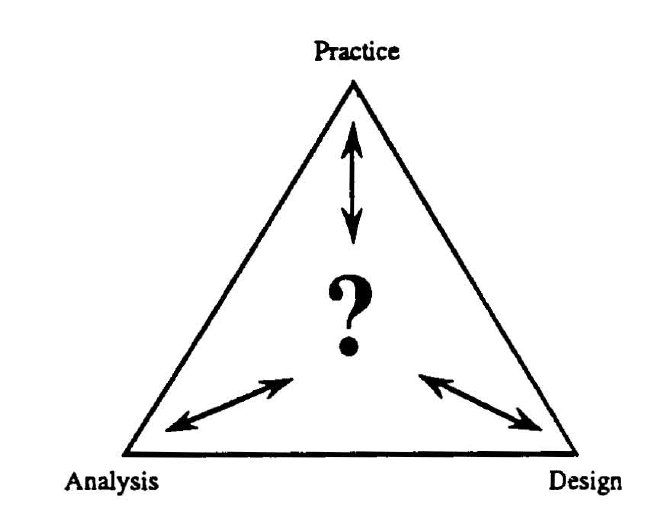
\includegraphics[scale=0.3]{Challenge_PD.jpg}
\caption{Hvordan kombinere alle?}
\label{Challenge_PD}
\end{figure}

\noindent
Ifølge \cite{Mogensen92} er det flere måter å oppnå større involvering av brukerene på. Én teknikk er fremtidsworkshops, der en ønsker en diskusjon rundt mulige fremtidige løsninger på nåværende problemer identifisert av brukerene selv. En annen teknikk er workshops hvor en bruker mock-ups og prototyper for å trigge diskusjonen om mulige fremtidige teknologier.  Uavhengig av valgt teknikk vil graden av relavans til dagens praksis være avgjørende for workshopens suksess. Felles for de to er at de tar i bruk kontekstuelle artefakter.

\noindent
Mogesen og Trigg (1992) konkluderer med at ved bruk av kontekstualiserte artefakter kan lede til nettopp et slikt ønsket samspill (figur \ref{Artifacts_PD}). De argumenterer for at bruk av artefakter under en workshop ikke bare gir innspill på design - deltagende design, men at de også kan trigge diskusjoner som gir utviklerene bedre innsyn i dagens praksis, problemer og workarounds - deltagende analyse. 

\noindent
Deltagende design på denne måten, med bruk av kontekstualiserte artefakter, gir derfor forskere/utviklere en dypere forståelse av hva som er problemområdene, og hvordan brukerene oppfatter dagens situasjon. Det gir også brukerene mulighet til å bli klar over egne arbeidsmetoder og workarounds.

\begin{figure}[H]
\centering
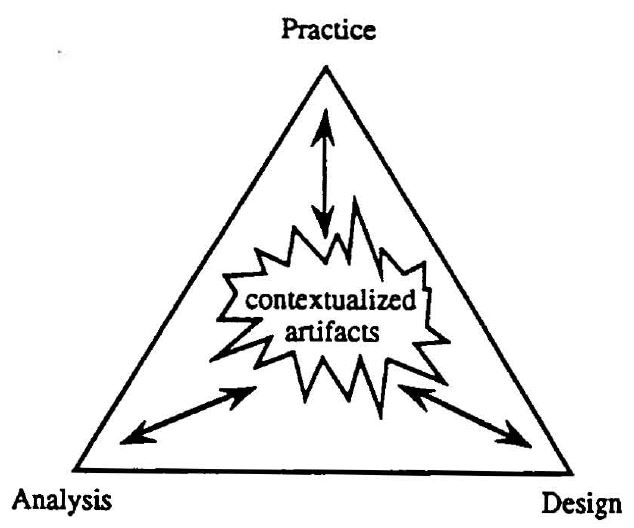
\includegraphics[scale=0.3]{Artifacts_PD.jpg}
\caption{Kontekstuelle artefakter støtter samspillet mellom de tre perspektivene}
\label{Artifacts_PD}
\end{figure}